\documentclass{standalone}
\usepackage{tikz}
\usetikzlibrary{arrows.meta, bending, positioning, intersections, backgrounds}
\tikzset{x=0.6cm,y=0.6cm, >={Stealth[bend]}}

\begin{document}  
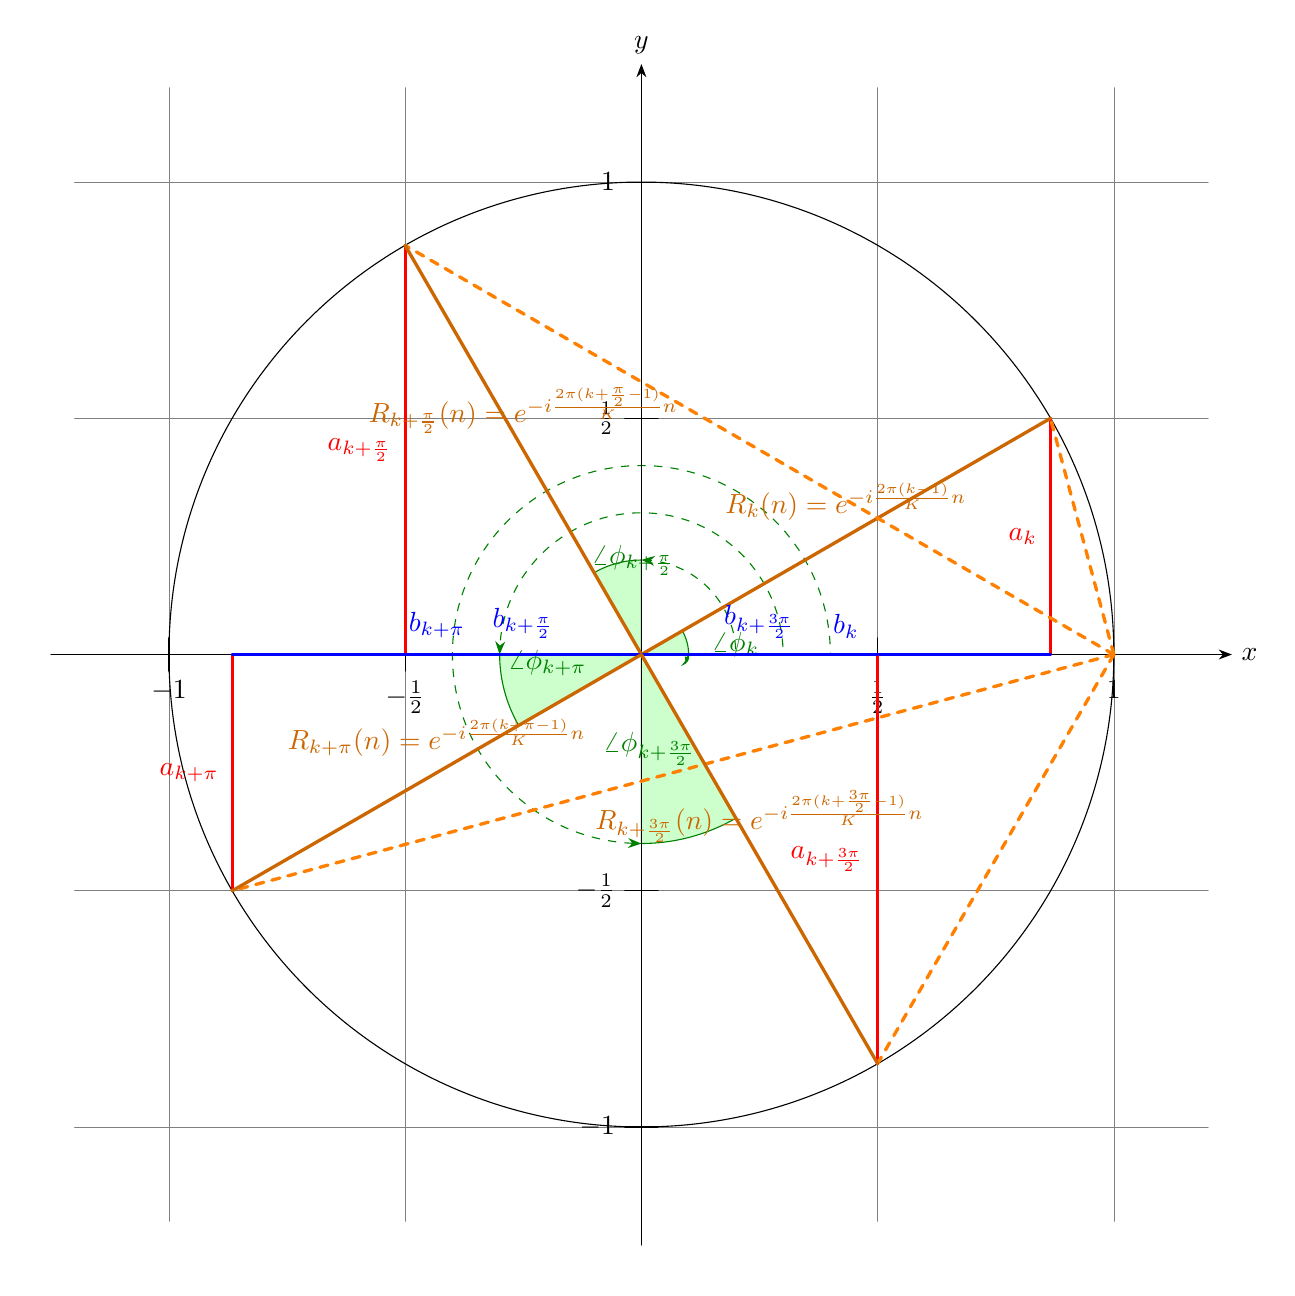
\begin{tikzpicture} 
% Style
[
    scale=6, line cap=round, axes/.style=,
    important line/.style={very thick},
    information text/.style={rounded corners,fill=red!10,inner sep=1ex}
]

% Define: Colors
\colorlet{shadow}{white!00}
\colorlet{angle_cover}{green!20}
\colorlet{angle_color}{green!50!black}
\colorlet{amplitude}{orange!80!black}
\colorlet{sin_color}{red}
\colorlet{cos_color}{blue}

%================================== Prepare ==================================
\def\foo draw_complex_exponential#1#2#3#4{
    % Draw: Angle-#1~#2
    \begin{scope}[on background layer]
        \draw [dashed, angle_color, ->] { 
            (0,0) -- (0:#4) arc [start angle=0, end angle=#1, radius=#4]
        };
        \filldraw [fill=angle_cover, draw=angle_color] { 
            (0,0) -- (#1:#4) arc [start angle=#1, end angle=#2, radius=#4]
        };
    \end{scope}
    
    % Draw: sin_cos
    \draw (#1+5:2mm) node[angle_color] {$\angle\phi_{#3}$};
    \draw [important line, sin_color] {
        (#2:1cm) -- 
            node[left =1pt] {$a_{#3}$} 
        (#2:1cm |- x axis)
    };
    \draw [important line, cos_color] {
        (#2:1cm |- x axis) -- 
            node[above=2pt] {$b_{#3}$} 
        (0,0)
    };

    % Draw: Calculate line-cross
    \path [name path=circle_holder] (0,0) circle [radius = 1cm];
    \path [name path=line_upward] (1.0cm, 0) -- (1.0cm, 1.0cm);
    \path [name path=line_sloped] (0.0cm, 0) -- (#2:1.5cm);
    \draw [name intersections={of=circle_holder and line_sloped, by=p}]
        [very thick, dashed, orange] {
        (1.0cm,0) -- 
            % node [right=1pt] {
            %     $\angle\phi_{\omega} = \frac{\color{red}\sin \alpha}{\color{blue}\cos \alpha}$
            % } 
        (p)
    };
    \draw [important line, amplitude] {
        (0,0) -- 
            node[above=2pt] {$R_{#3}(n) = e^{-i \frac{2\pi ({#3}-1)}{K} n}$} 
        (p)
    };
}

%=================================== Start ===================================
{
    % Define: Axis
    \draw [help lines, step = 0.5cm] (-2.0, -2.0) grid (2.0, 2.0);
    \begin{scope}[axes]
        \draw[->] (-1.25cm, 0) -- (1.25cm, 0) node[right] {$x$} coordinate(x axis);
        \draw[->] (0, -1.25cm) -- (0, 1.25cm) node[above] {$y$} coordinate(y axis);
        \foreach \x/ \xtext in {-1, -0.5/-\frac{1}{2}, 0.5/\frac{1}{2}, 1} {
            \draw[xshift=\x cm] (0pt, 1pt) -- (0pt, -1pt) node[below] {$\xtext$};
        }
        \foreach \y/ \ytext in {-1, -0.5/-\frac{1}{2}, 0.5/\frac{1}{2}, 1} {
            \draw[yshift=\y cm] (1pt, 0pt) -- (-1pt, 0pt) node[left ] {$\ytext$};
        }
    \end{scope}

    % Draw: Circle
    \draw (0,0) circle [radius = 1cm];
    
    % Draw: Rectangle-90
    \foo draw_complex_exponential{01} {30} {k}                {1mm}
    \foo draw_complex_exponential{90} {120}{k+\frac{\pi}{2}}  {2mm}
    \foo draw_complex_exponential{180}{210}{k+\pi}            {3mm}
    \foo draw_complex_exponential{270}{300}{k+\frac{3\pi}{2}} {4mm}

    % Draw: Rectangle-180
    % \foo draw_complex_exponential{01} {30} {k}                {1mm}
    % \foo draw_complex_exponential{180}{210}{k+\pi}            {3mm}
}
%==================================== END ====================================
\end{tikzpicture}
\end{document}